\documentclass[xcolor={dvipsnames}]{beamer}
\usepackage{color, colortbl}
\usepackage[ngerman,english]{babel}
\usepackage[T1]{fontenc}
\usepackage{CJKutf8} %japanese
\usepackage{lmodern}
%\usepackage{subfigure}
\usepackage[compatibility=false]{caption}
\usepackage{subcaption}
\usepackage{tikz}
\usepackage{textgreek}
\usepackage{tabularx}
\usepackage{ragged2e}
\usepackage{adjustbox}
\usepackage{booktabs}
\usepackage{siunitx}
\usepackage{units}
\usepackage{appendixnumberbeamer}
\usepackage[absolute,overlay]{textpos} %for positioning the logos where I want

\usepackage{animate}
\usepackage{multimedia}
\usepackage{fixltx2e}
\usepackage{multicol}
\usepackage{comment}
\DeclareSIUnit\year{yr}

\mode<presentation>
{
  \usetheme{CambridgeUS}     
  \usecolortheme{lily} 
  \definecolor{beamer@violet}{rgb}{0.5,0.3,0.5} % changed this
  \setbeamercolor{structure}{fg=beamer@violet!70!cyan}
  \setbeamercolor{palette primary}{fg=black, bg=gray!30!white!50!cyan!20!}
  \setbeamercolor{palette secondary}{fg=black, bg=gray!30!white!30!cyan!40!}
  \setbeamercolor*{palette tertiary}{bg=gray!20!white!20!cyan!60!}
  
  \setbeamercolor{frametitle}{fg=cyan!60!white!40!,bg=cyan!80!black}
  \setbeamercolor{title}{fg=cyan!80!black}
  \setbeamercolor{normal text}{fg=black,bg=white}
  \setbeamercolor{alerted text}{fg=beamer@violet}
  \setbeamercolor{example text}{fg=beamer@violet!70!cyan}
  
  \usefonttheme{structureitalicserif} 
  \setbeamertemplate{navigation symbols}{}
  \setbeamertemplate{caption}[numbered]
}
\newcommand{\sidlogo}{
  \setlength{\TPHorizModule}{1pt}
  \setlength{\TPVertModule}{1pt}
   % textblock{}{x,y}: pos(x) = rightUpperCorner + (x * \TPHorizModule), pos(y) = leftUpperCorner - (y * \TPVertModule)
  \begin{textblock}{1}(323,12)
   
\includegraphics[width=40pt,height=26pt]{figures/SiD.jpeg}
  \end{textblock}
  } 
\newcommand{\ilclogo}{
  \setlength{\TPHorizModule}{1pt}
  \setlength{\TPVertModule}{1pt}
   % textblock{}{x,y}: pos(x) = rightUpperCorner + (x * \TPHorizModule), pos(y) = leftUpperCorner - (y * \TPVertModule)
  \begin{textblock}{1}(323,12)
   
\includegraphics[width=40pt,height=26pt]{figures/ILC.jpeg}
  \end{textblock}
} 
\newcommand{\ejadelogo}{
  \setlength{\TPHorizModule}{1pt}
  \setlength{\TPVertModule}{1pt}
   % textblock{}{x,y}: pos(x) = rightUpperCorner + (x * \TPHorizModule), pos(y) = leftUpperCorner - (y * \TPVertModule)
  \begin{textblock}{1}(323,12)
   
\includegraphics[width=40pt,height=26pt]{figures/EJADE.jpeg}
  \end{textblock}
} 
\newcommand{\ATFlogo}{
  \setlength{\TPHorizModule}{1pt}
  \setlength{\TPVertModule}{1pt}
   % textblock{}{x,y}: pos(x) = rightUpperCorner + (x * \TPHorizModule), pos(y) = leftUpperCorner - (y * \TPVertModule)
  \begin{textblock}{1}(323,12)
   
\includegraphics[width=40pt,height=26pt]{figures/ATF_logo.jpg}
  \end{textblock}
} 
\newcommand{\RHULlogo}{
  \setlength{\TPHorizModule}{1pt}
  \setlength{\TPVertModule}{1pt}
   % textblock{}{x,y}: pos(x) = rightUpperCorner + (x * \TPHorizModule), pos(y) = leftUpperCorner - (y * \TPVertModule)
  \begin{textblock}{1}(337,12)
   
\includegraphics[width=25pt,height=26pt]{figures/rhul_logo.png}
  \end{textblock}
}
\newcommand{\flukalogo}{
  \setlength{\TPHorizModule}{1pt}
  \setlength{\TPVertModule}{1pt}
   % textblock{}{x,y}: pos(x) = rightUpperCorner + (x * \TPHorizModule), pos(y) = leftUpperCorner - (y * \TPVertModule)
  \begin{textblock}{1}(315,12)
   
\includegraphics[width=60pt,height=26pt]{figures/fluka_logo.png}
  \end{textblock}
} 

\newcommand{\paper}{
  \setlength{\TPHorizModule}{1pt}
  \setlength{\TPVertModule}{1pt}
   % textblock{}{x,y}: pos(x) = rightUpperCorner + (x * \TPHorizModule), pos(y) = leftUpperCorner - (y * \TPVertModule)
  \begin{textblock}{65}(256,12)
  \centering
  \textblockcolour{SpringGreen}
  \vspace*{0.8mm}{arXiv:\\1609.07816v1}\vspace*{0.8mm}
  \end{textblock}
} 

\newcommand{\proceedigHelix}{
  \setlength{\TPHorizModule}{1pt}
  \setlength{\TPVertModule}{1pt}
   % textblock{}{x,y}: pos(x) = rightUpperCorner + (x * \TPHorizModule), pos(y) = leftUpperCorner - (y * \TPVertModule)
  \begin{textblock}{55}(266,12)
  \centering
  \textblockcolour{SpringGreen}
  \vspace*{0.8mm}{arXiv:\\1703.05737}\vspace*{0.8mm}
  \end{textblock}
} 

\newcommand{\proceedigBDS}{
  \setlength{\TPHorizModule}{1pt}
  \setlength{\TPVertModule}{1pt}
   % textblock{}{x,y}: pos(x) = rightUpperCorner + (x * \TPHorizModule), pos(y) = leftUpperCorner - (y * \TPVertModule)
  \begin{textblock}{55}(266,12)
  \centering
  \textblockcolour{SpringGreen}
  \vspace*{0.8mm}{arXiv:\\1703.05738}\vspace*{0.8mm}
  \end{textblock}
} 

\newcommand{\electron}{e$^-$}
\newcommand{\positron}{e$^+$}

\title[ILC \& Background Simulations]{\textbf{\LARGE The International Linear Collider \\ \large Background Simulations \& the Impact on SiD}}
\author[Anne Sch\"utz]{\underline{Anne Sch\"utz} \inst{1}, M. Stanitzki \inst {1}, J. Strube \inst{2}, B. Schumm \inst{3}, C. Milke \inst{3}, L. d`Hautuille \inst{3}, G. White \inst{4}, L. Keller \inst{4}, T. Barklow \inst{4}\\
\& SiD Optimization Group}

\institute[DESY]{\inst{1} DESY \inst{2} PNNL \inst{3} UCSC \inst{4} SLAC}
\date[May 1st 2017]{May 1st 2017\\\textbf{LC Vertex Detector Workshop 2017}}

\titlegraphic{

\includegraphics[height=1.2cm]{figures/DESY_Logo.png}\hspace*{1cm}~%
\includegraphics[height=1.2cm]{figures/PNNL_Logo.png}\hspace*{1cm}~%

\includegraphics[height=1.2cm]{figures/SiD.jpeg}\hspace*{1cm}~%
\includegraphics[height=1.2cm]{figures/UCSC_Logo.png}\hspace*{1cm}~%
\includegraphics[height=1.2cm]{figures/SLAC_Logo.png}
}

\begin{document}

\begin{frame}
\begin{center}
\LARGE Additional Material
\end{center}
  \tableofcontents
\end{frame}

\section{ILC}
\subsection{ILC parameters}

%------Definition for column color in table
\definecolor{Gray}{gray}{0.9}
\newcolumntype{g}{>{\columncolor{Gray}}r}
%-----------------------------------------
\begin{frame}{The beam parameters of the ILC}
\ilclogo

\begin{table}[]
\centering
\begin{tabularx}{\textwidth}{ll|rrrg}
\hline
& & \multicolumn{1}{>{\centering}p{1.5cm}}{\textbf{Baseline 500}} & \multicolumn{1}{>{\centering}p{1.5cm}}{\textbf{Lumi Upgrade}} & \multicolumn{1}{>{\centering}p{1.5cm}}{\textbf{TeV Upgrade}} & {\centering\textbf{LHC 25ns}} \\ 
\hline
\cline{1-6}
\hline
E$_{CM}$  &[\si{\GeV}] & 500  & 500  & \num{1000} & \num{14000}\\
n$_b$ & & \num{1312} & \num{2625} & \num{2450} &  \num{2808} \\
$\Delta t_b$ &[\si{\nano\second}] & 554  & 366   & 366 & 25 \\
N & & \num{2.0e10}  & \num{2.0e10}  & \num{1.74e10}  & \num{11.5e10}\\
q$_b$ &[\si{\nano\coulomb}] & 3.2  & 3.2  &  2.7 & 18.4 \\
$\sigma_x^*$ &[\si{\nano\metre}] & 474  & 474  &  481 & \num{16700}\\
$\sigma_y^*$ &[\si{\nano\metre}] & 5.9 &  5.9  &  2.8 & \num{16700}\\
$\sigma_z$ &[\si{\milli\metre}] & 0.3  &  0.3  &  0.25 & 0.755\\
L &[\si{\per\centi\metre\squared\per\second}] & \num{1.8e34} & \num{3.6e34} & \num{3.6e34} & \num{1.0e34}\\
\hline
\end{tabularx}
\end{table}
\end{frame}
\begin{frame}{ILC baseline parameters}
\ilclogo
\centering
\includegraphics[width=1.01\textwidth]{figures/ILC_running_scenarios_parameters.png}
%	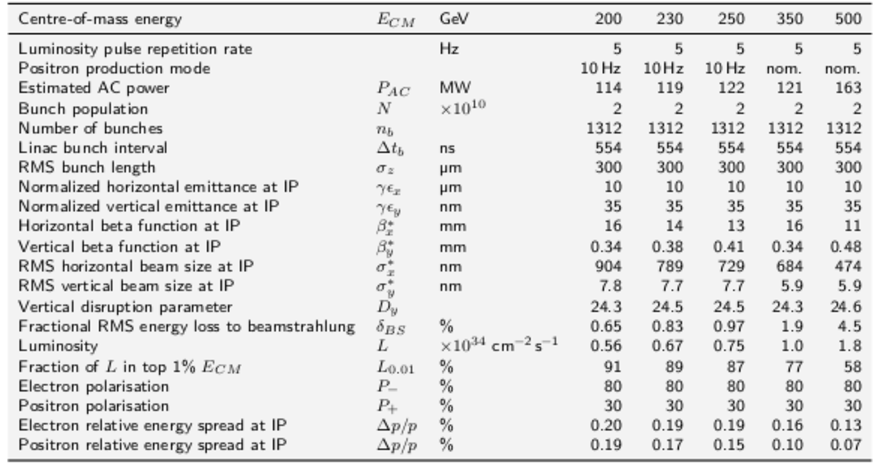
\includegraphics[width=\textwidth]{figures/ILCTDR-VOLUME_3-PART_II_ILCparameters.pdf}
\end{frame}
%\begin{frame}{ILC parameters for the different upgrade stages}
%\ilclogo
%\centering
%	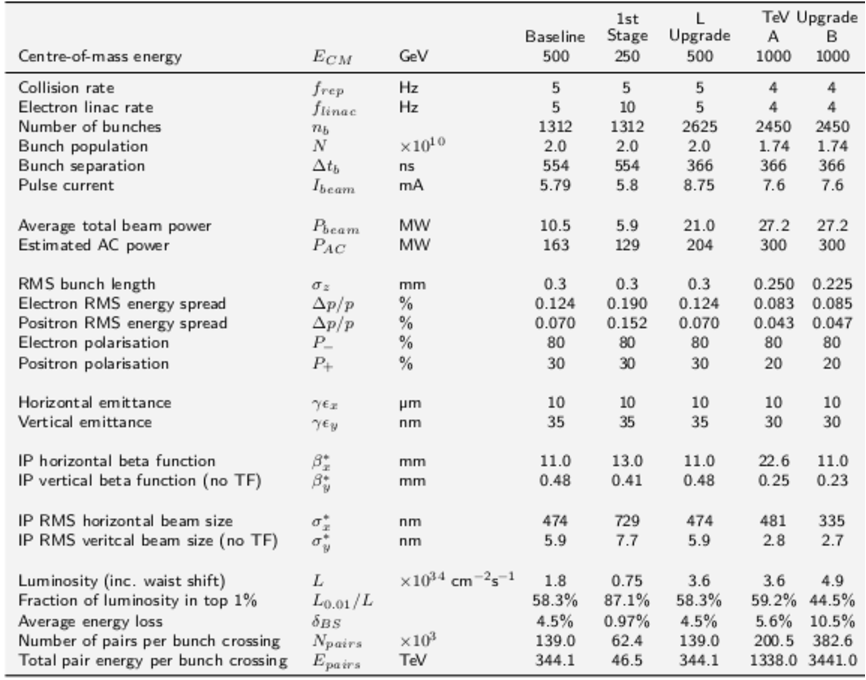
\includegraphics[width=0.8\textwidth]{figures/ILCTDR-VOLUME_3-PART_II_ILCparametersUpgrades.pdf}
%\end{frame}

\AtBeginSection[] {
  \begin{frame}<beamer>
     \tableofcontents[currentsection,
     currentsubsection,
     %hideothersubsections,
     subsectionstyle=show/show/hide,
     subsubsectionstyle=show/show/hide]
  \end{frame}
}

\section{SiD - Subdetector Specifications}
\begin{frame}
 \begin{table}
\caption{Key parameters of the baseline SiD design, including the measurements of the subdetectors, and their readout cell dimensions. The given readout cell dimension are the pixelation cell sizes used for the full detector Geant4 simulation.}
\label{tab:KeyParametersSiD}
\begin{tabular}{>{\raggedright}p{1.8cm}>{\raggedright}p{2.4cm}>{\raggedright}p{2.2cm}>{\centering}p{1.2cm}>{\raggedright}p{1.2cm}>{\raggedright}p{1.2cm}>{\raggedright}p{1.2cm}}
\hline\hline
\textbf{SiD Barrel} & \textbf{Technology} & \textbf{Readout cell dimensions [mm$^2$]} & \textbf{Inner radius [cm]} & \textbf{Outer radius [cm]} & \textbf{z extent [cm]} \tabularnewline
\hline
Vertex detector & Silicon pixels & 0.05 x 0.05 & 1.4 & 6.0 & $\pm 6.25$ \tabularnewline
Tracker & Silicon strips & 0.05 x 0.05 & 21.7 & 122.1 & $\pm 152.2$ \tabularnewline
ECAL & Silicon pixels- W & 3.5 x 3.5 & 126.5 & 140.9 & $\pm 176.5$ \tabularnewline
HCAL & RPC - steel & 10 x 10 & 141.7 & 249.3 & $\pm 301.8$ \tabularnewline
Solenoid & 5 T SC & - & 259.1 & 339.2 & $\pm 298.3$ \tabularnewline
Flux return & Scintillator- steel & 30 x 30 & 340.2 & 604.2 & $\pm 303.3$ \tabularnewline
\hline
\end{tabular}
\end{table}
\end{frame}

\begin{frame}
 \begin{table}
\begin{tabular}{>{\raggedright}p{1.8cm}>{\raggedright}p{2.4cm}>{\raggedright}p{2.2cm}>{\centering}p{1.2cm}>{\raggedright}p{1.2cm}>{\raggedright}p{1.2cm}>{\raggedright}p{1.2cm}}
\hline\hline
\textbf{SiD Endcap} & \textbf{Technology} & \textbf{Readout cell dimensions [mm$^2$]} & \textbf{Inner z [cm]} & \textbf{Outer z [cm]} & \textbf{Outer radius [cm]} \tabularnewline
\hline
Vertex detector & Silicon pixels & 0.05 x 0.05 & 7.3 & 83.4 & 16.6 \tabularnewline
Tracker & Silicon strips & 0.05 x 0.05 & 77.0 & 164.3 & 125.5 \tabularnewline
ECAL & Silicon pixel- W & 3.5 x 3.5 & 165.7 & 180.0 & 125.0 \tabularnewline
HCAL & RPC - steel & 10 x 10 & 180.5 & 302.8 & 140.2 \tabularnewline
Flux return & Scintillator- steel & 30 x 30 & 303.3 & 567.3 & 604.2 \tabularnewline
LumiCal & Silicon- W & 3.5 x 3.5 & 155.7 & 169.55 &  20.0 \tabularnewline
BeamCal & Semicond.- W & 3.5 x 3.5 & 326.5 & 344 & 14.0 \tabularnewline
\hline\hline
\end{tabular}
\end{table}
\end{frame}

\section{Background from High Cross Section ILC Processes}
\subsection{FCAL Occupancy}
\begin{frame}{Occupancy in the FCAL}
  \begin{center}
     \includegraphics[width=0.7\textwidth]{figures/fig_raw_occupancy.png}
  \end{center}
  Number of hits per channel during a full ILC bunch train ($\sim$2600 bunch crossings).\\
  {\hfill \tiny Study done by B. Schumm and students at UCSC}
\end{frame}

\AtBeginSubsection[] {
  \begin{frame}<beamer>
     \tableofcontents[currentsection,
     currentsubsection,
     %hideothersubsections,
     subsectionstyle=show/shaded/hide,
     subsubsectionstyle=show/show/hide]
  \end{frame}
}
\subsection{Pair background timing}
\begin{frame}{Creation time of particles hitting the Vertex Detector}
\begin{columns}
 \begin{column}{0.5\textwidth}
Distribution of the time of creation (relative to the bunch crossing) of pair background particles (from 1312 bunches) that hit the endcaps of the VXD.
At the time of the bunch crossing about \num{1.6e6} particles are created (underflow bin).\\
 {\footnotesize The creation time is plotted for pair background particles hitting the vertex endcaps only. This is to avoid double counting of particles that would hit both, the barrel and the endcaps.}
 \end{column}
 \begin{column}{0.55\textwidth}
 \includegraphics[width=1\textwidth]{figures/creationtime_histo_SiVertexEndcap_SiDNote.pdf}
 \end{column}
\end{columns}
 %\adjustbox{max height=\dimexpr\textheight-5.5cm\relax,
%           max width=\textwidth}{
\begin{table}
\footnotesize
\begin{tabular}{>{\RaggedRight}p{1.8cm}>{\RaggedRight}p{1.9cm}>{\RaggedRight}p{1.7cm}>{\RaggedRight}p{2.4cm}>{\RaggedRight}p{2.3cm}}
Overall pairs & Primary pairs [\unit[0]{ns};\unit[11]{ns}] & Late pairs ]\unit[11]{ns};\unit[50]{ns}] & Out-of-time backscatter pairs ]\unit[50]{ns};\unit[554]{ns}] & Out-of-time backscatter pairs ]\unit[554]{ns};\unit[1000]{ns}]\\
\hline
$\sim$ \num{1.9e6} & 87.33\% & 12.38\% & 0.16\% &  0.029\% 
\end{tabular}
\end{table}
%}
\end{frame}

\begin{frame}{Momentum distribution particles hitting the Vertex Detector}
  \includegraphics[width=0.5\textwidth]{figures/momentum_histo_SiVertexBarrelSiVertexEndcap_SiDNote.pdf}
  \includegraphics[width=0.5\textwidth]{figures/transvmomentum_histo_SiVertexBarrelSiVertexEndcap_SiDNote}\\
  Distributions of the pair background particle momenta of pair background particles from 1312 bunches that will hit the barrel and the endcaps of the vertex detector.
  The plots show the histograms of the total and the transverse momenta of the particles hitting the vertex detector, in certain time intervals.
\end{frame}

\subsection{Pair background helixes}
\begin{frame}{Comparison of P\textsubscript{T} and P\textsubscript{z} of the ILC pairs}
Comparison between pairs from ILC \textbf{500}, \textbf{\textcolor{Red}{350}} and \textbf{\textcolor{Blue}{250}\,GeV}\\
\vspace*{0.5cm}
  \includegraphics[width=0.5\textwidth]{figures/pairs_comparison_PT.png}
  \includegraphics[width=0.5\textwidth]{figures/pairs_comparison_Pz.png}
\end{frame}

\begin{frame}{P\textsubscript{T} vs. P\textsubscript{z} of the pairs from ILC 500, 350 and 250\,GeV}
\hspace*{1.4cm}500\,GeV \hspace*{2.5cm} 350\,GeV \hspace*{2.5cm} 250\,GeV\\
\vspace*{0.5cm}
  \includegraphics[width=0.34\textwidth]{figures/pairs500_PTvsPz.png}
  \includegraphics[width=0.34\textwidth]{figures/pairs350_PTvsPz.png}
  \includegraphics[width=0.34\textwidth]{figures/pairs250_PTvsPz.png}
\end{frame}


\begin{frame}{Explanation of helix track calculations}
\proceedigHelix
 \begin{center}
  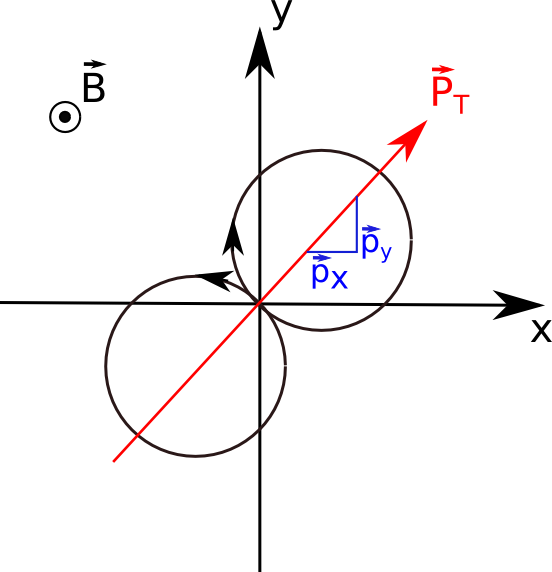
\includegraphics[width=0.65\textwidth]{figures/Helix_explanation.png}
\end{center}
\end{frame}

\section{Muons from the BDS}
\begin{frame}{The Muons in SiD - Spatial Distribution}
\proceedigBDS
 \includegraphics[width=0.9\textwidth]{figures/Explanation_Spatial_distribution_NEW.pdf}
\end{frame}

\begin{frame}{The Muon Occupancy in SiD}
\proceedigBDS
 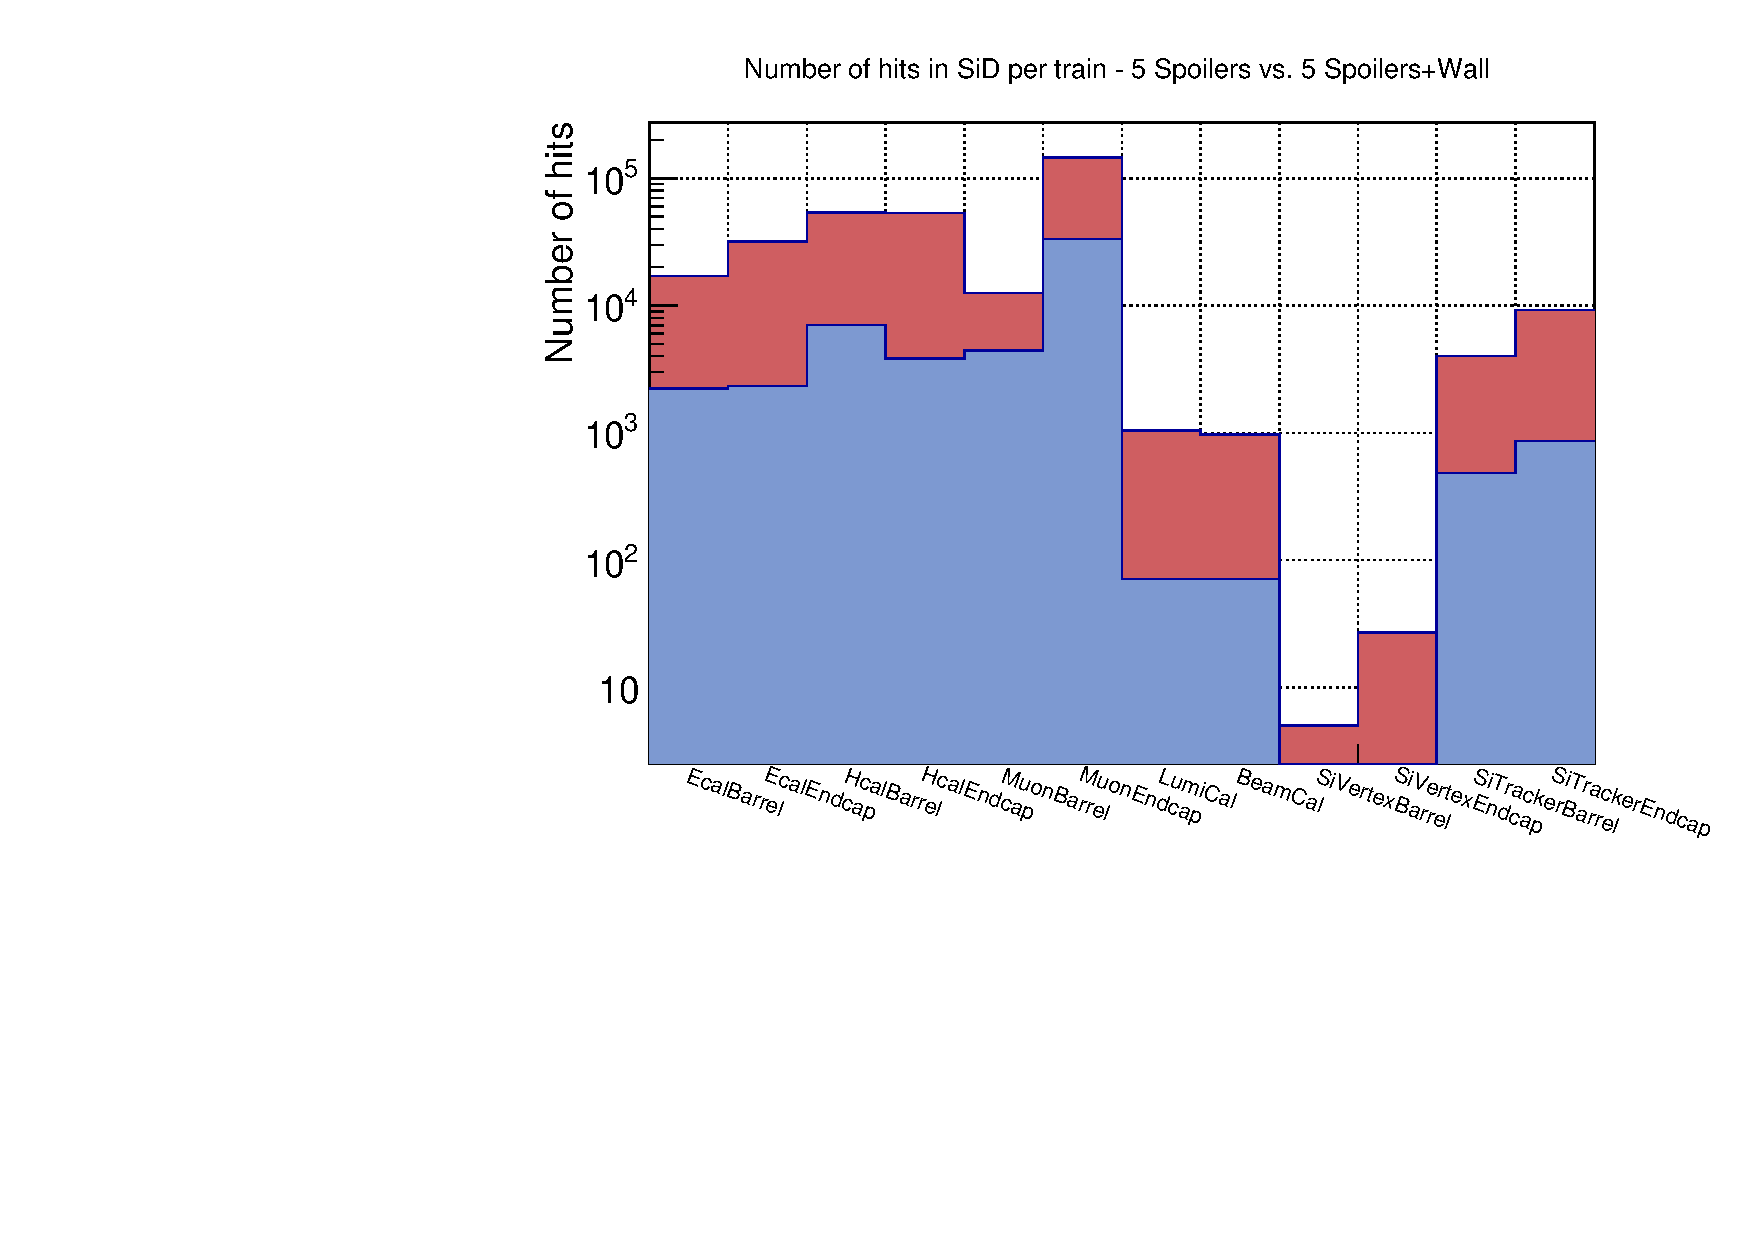
\includegraphics[width=0.6\textwidth]{figures/Hits_in_SiD_subdetectors_MuonSpoilerStudy.pdf}
  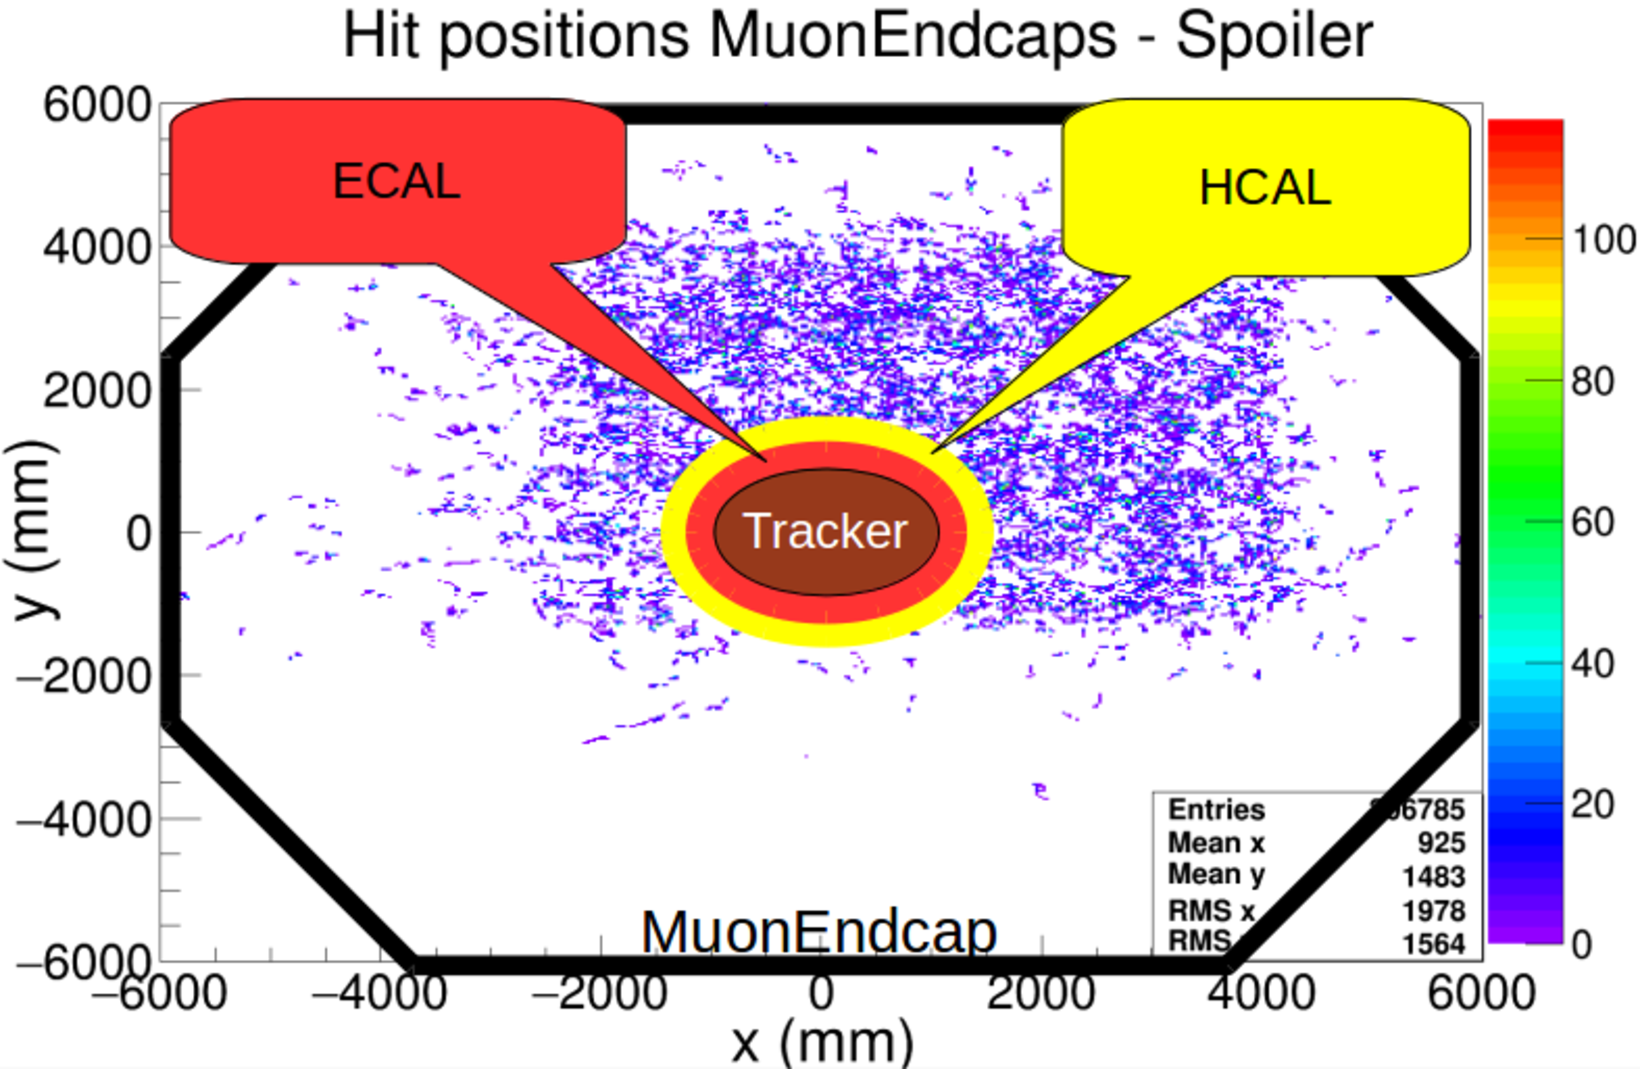
\includegraphics[width=0.45\textwidth]{figures/Explanation_Hits_Subdetectors.pdf}\\
The number of hits in the different SiD subdetectors for both shielding scenarios (\textcolor{Red}{``5 Spoilers''} and \textcolor{Blue}{``5 Spoilers + Wall''}) is not evenly distributed.\\
The number of hits depends on the effective area of the subdetector system.
 \end{frame}
 
 \begin{frame}{Muon Occupancy in SiD HCAL endcaps}
 \proceedigBDS
  \includegraphics[width=0.53\textwidth]{figures/muon_occupancy_deadcells_all_layers_HcalBarrel.pdf}
  \includegraphics[width=0.53\textwidth]{figures/muon_occupancy_deadcells_all_layers_HcalEndcap.pdf}\\
The current SiD electronics design has a \textcolor{Green}{buffer depth of 4}:\\
$\sim$\textcolor{Blue}{1$\times$10\textsuperscript{-6}} - \textcolor{Red}{4$\times$10\textsuperscript{-6}} of all hits are dead in the \textbf{HCAL barrel}\\
$\sim$\textcolor{Blue}{2$\times$10\textsuperscript{-4}} - \textcolor{Red}{1$\times$10\textsuperscript{-3}} of all hits are dead in the \textbf{HCAL endcaps}
\end{frame}

\begin{frame}{Muon Occupancy in SiD Tracker endcaps}
\proceedigBDS
\begin{center}
  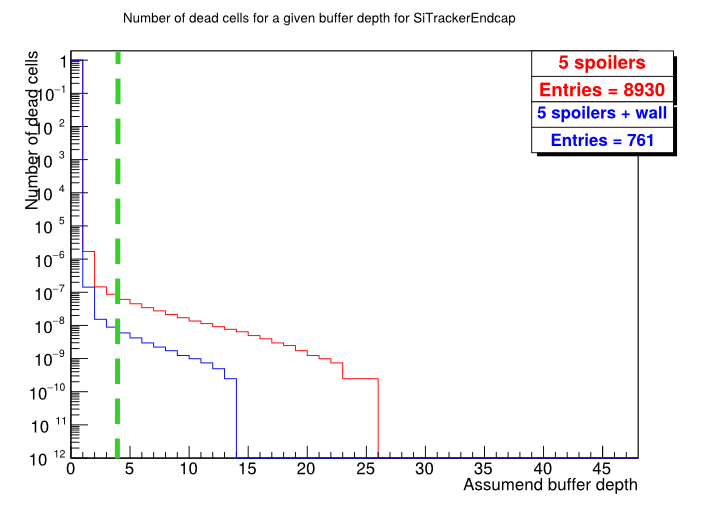
\includegraphics[width=0.65\textwidth]{figures/SiTrackerEndcap_DeadCells.png}
\end{center}
The current SiD electronics design has a \textcolor{Green}{buffer depth of 4}, i.e. \textcolor{Blue}{10\textsuperscript{-8}} - \textcolor{Red}{10\textsuperscript{-7}} of all hits are dead in the Tracker endcaps.
\end{frame}
 
\begin{frame}{The Muon Energy}
\proceedigBDS
\begin{center}
  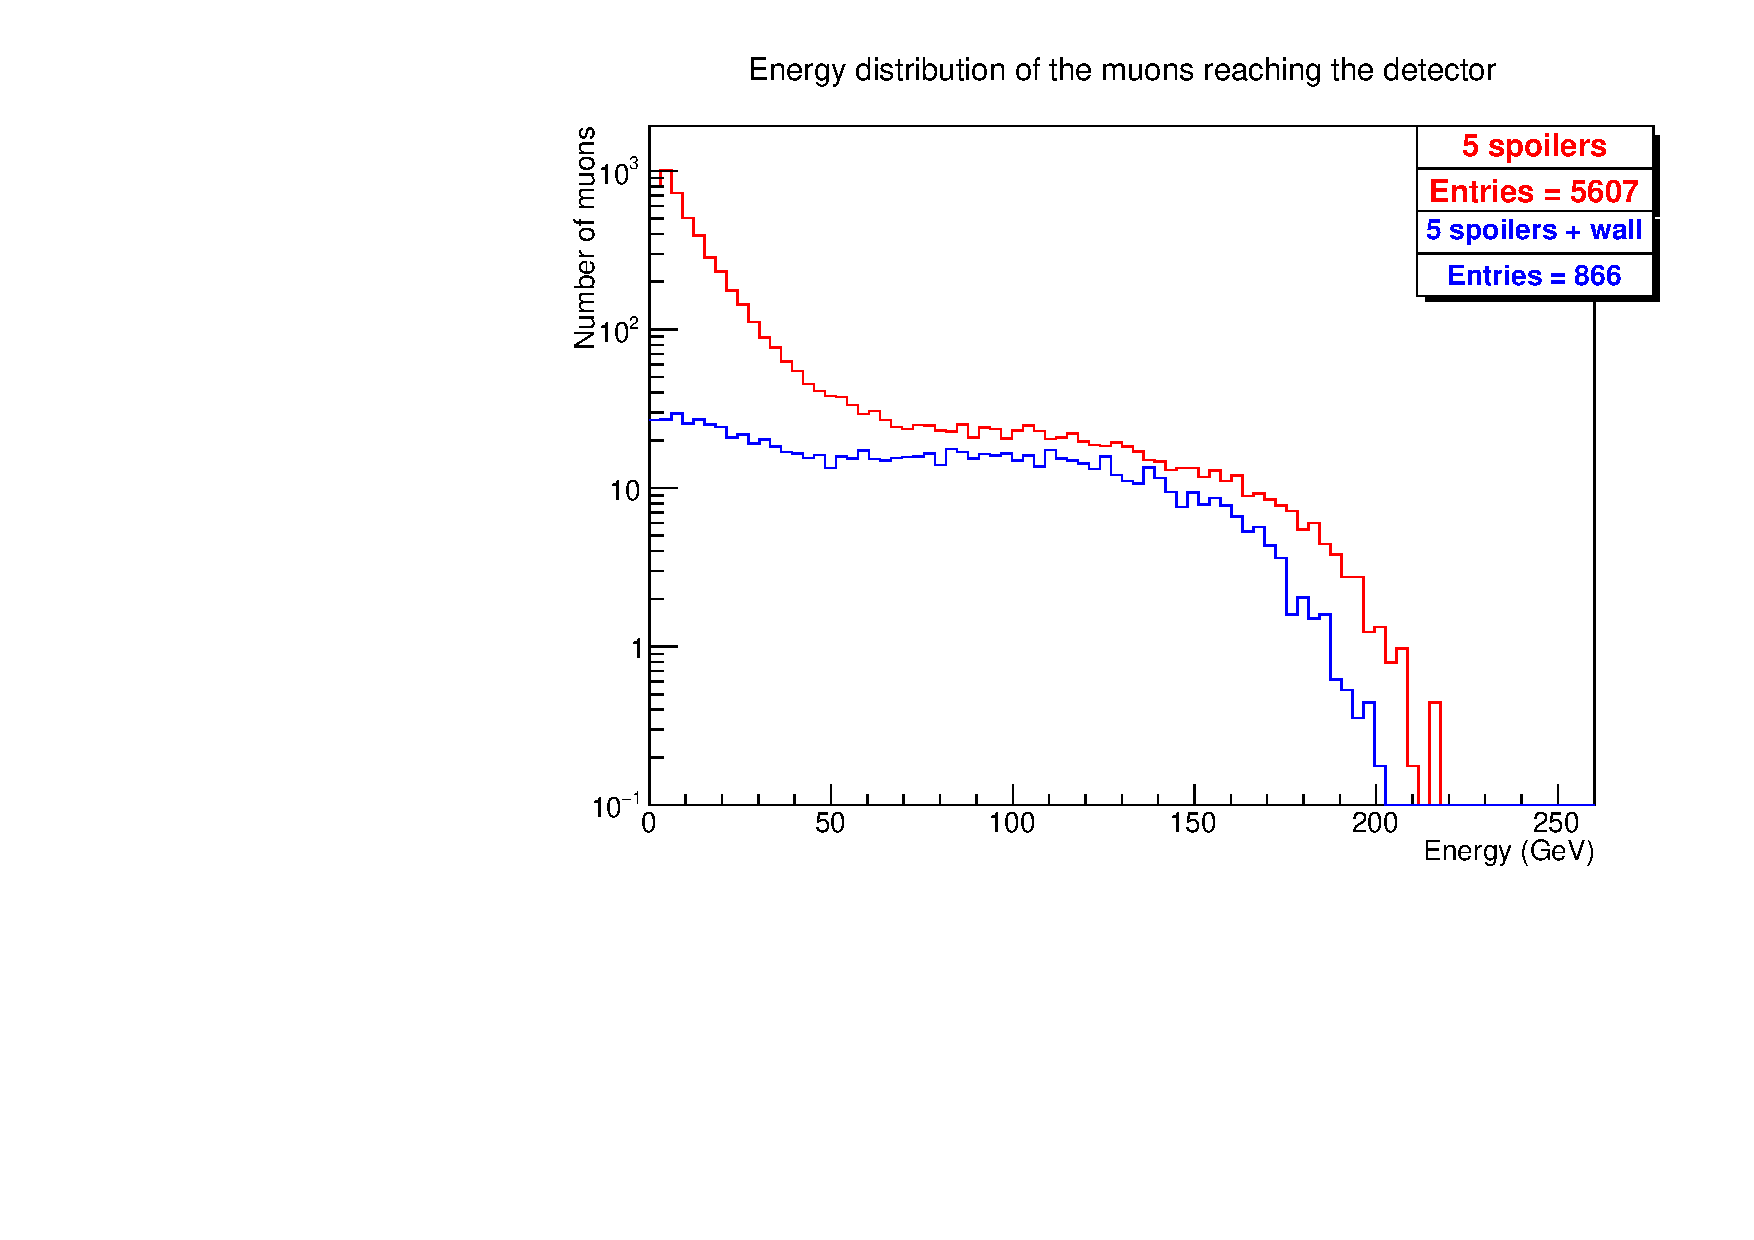
\includegraphics[width=0.65\textwidth]{figures/muon_energy.pdf}
\end{center}
The energy distribution of the muons from the ``5 Spoilers + Wall'' scenario does not reach the same maximum energy. The muons are decelerated and stopped within the magnetized wall.
\end{frame}

\end{document}